%%%%%%%%%%%%%%%%%%%%%%%%%%%%%%%%%%%%%%%%%%%%%%%%%%%%%%%%%%%%%%%%%%%%%%%%%%%%%%%%
% Лабораторная работа 6 : Статически определимая балка

% Выполнили             : Баталов Семен, Хайретдинова Диана, 2021.
%%%%%%%%%%%%%%%%%%%%%%%%%%%%%%%%%%%%%%%%%%%%%%%%%%%%%%%%%%%%%%%%%%%%%%%%%%%%%%%%

\documentclass[12pt, a4paper]{article}
\usepackage[left=1.5cm, right=2cm, top=2.5cm, bottom=2.5cm, nohead]{geometry}
\usepackage{graphicx}
\usepackage[utf8]{inputenc}
\usepackage[english, russian]{babel}
\usepackage{indentfirst}
\usepackage{amsmath}
\usepackage{longtable}
\usepackage{multirow}
\usepackage{array}
\usepackage{rotating}
\usepackage{subcaption}
\graphicspath{{./Pictures/}}

\begin{document}
    
    \newcolumntype{M}[1]{>{\centering\arraybackslash}m{#1}}
    \renewcommand{\arraystretch}{1.3}
    
    \begin{center}
        \large{Санкт-Петербургский Государственный Университет} \\
        \large{Saint-Petersburg State University}\\
        \hfill \break
        \hfill \break
        \hfill \break
        \hfill \break
        \hfill \break
        \hfill \break
        \large{ЛАБОРАТОРИЯ ПРОЧНОСТИ МАТЕРИАЛОВ} \\
        \hfill \break
        \hfill \break
        \hfill \break
        \large{\textbf{ОТЧЕТ}} \\
        \large{\textbf{По лабораторной работе 6}} \\
        \large{<<Определение линейных и угловых перемещений статически определимой балки >>} \\
        \hfill \break
        \hfill \break
        \hfill \break
        \large{По дисциплине} \\
        \large{<<Лабораторный практикум, лабораторная работа>>} \\
    \end{center}
    
    \hfill \break
    \hfill \break
    \hfill \break
    \hfill \break
    \hfill \break
    \hfill \break
    
    \begin{flushright} 
        \large{Выполнили:} \\
        \hfill \break
        \large{Баталов С. А.} \\
        \large{Хайретдинова Д. Д.} \\
    \end{flushright}
    
    \hfill \break
    \hfill \break
    \hfill \break
    \hfill \break
    \hfill \break
    
    \begin{center} 
        \large{Санкт-Петербург} \\
        \large{2021} \\
    \end{center}
    
    \thispagestyle{empty}
    \newpage
    \sloppy
    
    \section{Цель работы}
    Под изгибом понимают такой вид деформации, при котором в поперечных сечениях исследуемого образца возникают изгибающие моменты. Стержень, работающий на изгиб, называют балкой. Балка называется статически определимой, если все усилия и моменты в ней можно определить из уравнения статики. В частности, используемая в работе балка с одной шарнирно-подвижной и одной шарнирно-неподвижной опорами является статически определимой.
    
    При прямом поперечном изгибе ось бруса, искривляясь, остается в силовой плоскости. В результате деформации каждое из сечений занимает новое положение: их центры тяжести получают вертикальные и горизонтальные линейные перемещения, а сами сечения поворачивается на некоторый угол вокруг нейтральной оси.
    Гипотеза плоских сечений -- при повороте сечения остаются плоскими и перпендикулярными изогнутой оси балки.
    
    Цель работы заключается в измерении линейных и угловых перемещений, возникающих в статически определимой шарнирно закрепленной балке при изгибе ее сосредоточенной силой и сравнении измеренных величин с расчетными данными.
    
    \newpage
    \section{Теоретическое исследование}
    
    \newpage
    \section{Экспериментальная уствновка}
    
    \newpage
    \section{Эксперимент}
    
    \begin{figure}[h]
    	\centering
    	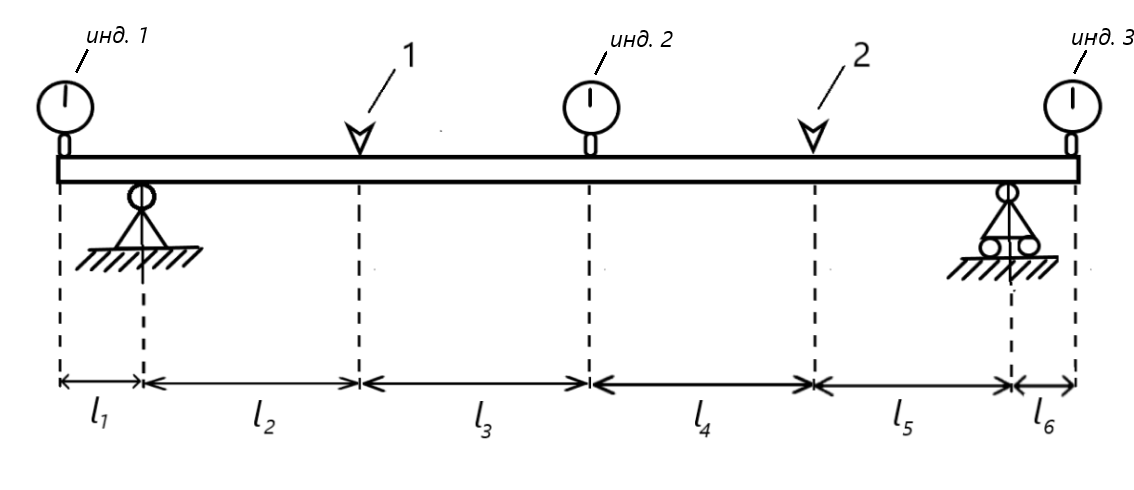
\includegraphics[width = 15cm]{pic_1.png}
    	\caption{Измерение длин балки}
    	\label{wow_picture}
    \end{figure}
    
    Измерили необходимые расстояния для 2 экспериментов: в 1-ом груз подвешен  в точке $1$, и во 2-ом груз подвешен в точке $2$, также замерили высоту $h$ и толщину $b$ балки с оценкой погрешности. \\
    \begin{table}[h]
    \centering
    
	\begin{tabular}{|M{2cm}|M{3cm}|M{3cm}|M{3cm}|}
	\hline
	Величина & Значение & Погрешность & Размерность \\
	\hline
	b & 5.4  & \multirow{2}{*}{$ \pm $0.1} & \multirow{8}{*}{мм} \\
	h & 36.1 & & \\
	\cline{1-3}
	$l_{1}$ & 80  & \multirow{6}{*}{$ \pm $1} & \\
	$l_{2}$ & 142 & & \\
	$l_{3}$ & 153 & & \\
	$l_{4}$ & 203 & & \\
	$l_{5}$ & 201 & & \\
	$l_{6}$ & 83  & & \\
	\hline
	\end{tabular}	    
    
    \label{tablichka}
	\caption{Начальные данные.}    
    \end{table}
    
	Далее провели 2 эксперимента, постепенно нагружая, затем разружая балку, снимали показания с индикаторных головок часового типа и занесли в таблицу, учитывая, что систематическая погрешность измерений $\Delta x = 10^{-2}$мм : 

	\newpage
    
    \begin{table}[h]
    \centering
    
    \begin{tabular}{|M{1cm}|M{1cm}|M{2cm}|M{2cm}|M{2cm}|M{2cm}|M{2cm}|M{2cm}|}
    \hline
    \multirow{4}{*}{№} & \multirow{3}{*}{P} & \multicolumn{3}{c|}{1 эксперимент} & \multicolumn{3}{c|}{2 эксперимент} \\
    \cline{3-8}
     & & \multicolumn{3}{c|}{Показания индикаторов} & \multicolumn{3}{c|}{Показания индикаторов} \\
     \cline{3-8}
     & & 1 & 2 & 3 & 1 & 2 & 3 \\
     \cline{2-8}
     & Н &\multicolumn{3}{c|}{$ \cdot 10^{-2} $ мм}& \multicolumn{3}{c|}{$\cdot 10^{-2} $ мм}\\
	 \hline
	 1 & 1 & 2 & -5 & 1 & 1 & -4 & 1 \\
	 2 & 2 & 5 & -10 & 3 & 4 & -12 & 5 \\
	 3 & 3 & 7 & -15 & 4 & 6 & -19 & 8 \\
	 4 & 5 & 12 & -26 & 7 & 10 & -32 & 14 \\
	 5 & 7 & 17 & -37 & 10 & 15 & -44 & 20 \\
	 6 & 12 & 28 & -63 & 18 & 25 & -76 & 34 \\
	 7 & 7 & 17 & -37 & 11 & 15 & -45 & 21 \\
	 8 & 5 & 12 & -27 & 7 & 11 & -33 & 15 \\
	 9 & 3 & 7 & -16 & 4 & 7 & -20 & 9 \\
	 10 & 2 & 5 & -11 & 3 & 4 & -13 & 6 \\
	 11 & 1 & 3 & -6 & 1 & 2 & -6 & 3 \\  
    \hline
    \end{tabular}
    
    \caption{Экспериментальные данные.}
    \end{table}
    
    \begin{table}[h]
    \centering
    
    \begin{tabular}{|M{1cm}|M{1cm}|M{2cm}|M{2cm}|M{2cm}|M{2cm}|M{2cm}|M{2cm}|}
    \hline
    \multirow{4}{*}{№} & \multirow{3}{*}{P} & \multicolumn{3}{c|}{1 эксперимент} & \multicolumn{3}{c|}{2 эксперимент} \\
    \cline{3-8}
     & & \multicolumn{3}{c|}{Показания индикаторов} & \multicolumn{3}{c|}{Показания индикаторов} \\
     \cline{3-8}
     & & 1 & 2 & 3 & 1 & 2 & 3 \\
     \cline{2-8}
     & Н &\multicolumn{3}{c|}{мкм??? 0.01}& \multicolumn{3}{c|}{мкм??? 0.01}\\
	 \hline
	 1 & 1 &  \\
	 2 & 2 &  \\
	 3 & 3 &  \\
	 4 & 5 &  \\
	 5 & 7 &  \\
	 6 & 12 & \\
    \hline
    \end{tabular}
    
    \caption{Экспериментальные данные.}
    \end{table}

 
\begin{figure}[h]
\centering
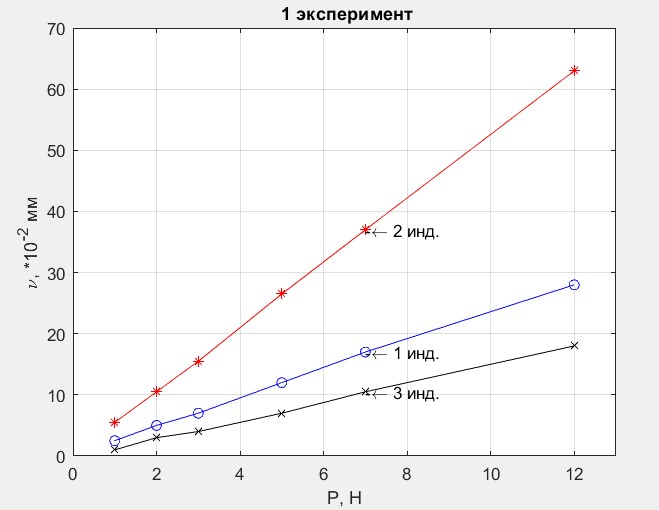
\includegraphics[width = 15cm]{nu_1.jpg}
\caption{Графики зависимости прогиба $\nu$ от нагрузки}
\label{nu_levoe}
\end{figure}

\begin{figure}[h]
\centering
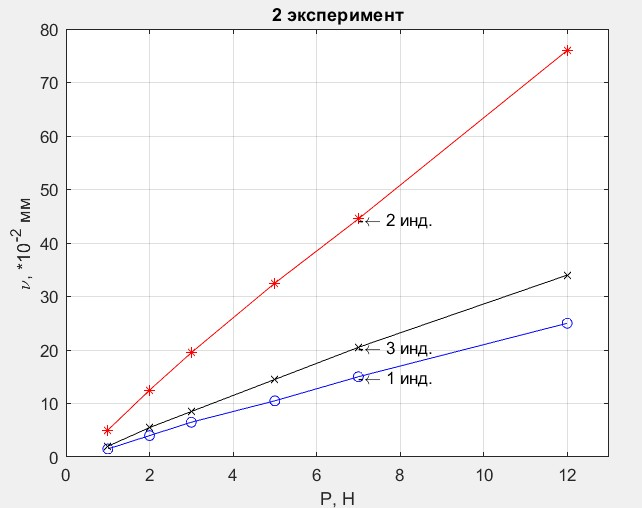
\includegraphics[width = 15cm]{nu_2.jpg}
\caption{Графики зависимости прогиба $\nu$ от нагрузки}
\label{nu_pravoe}
\end{figure}

\begin{figure}[h]
\centering
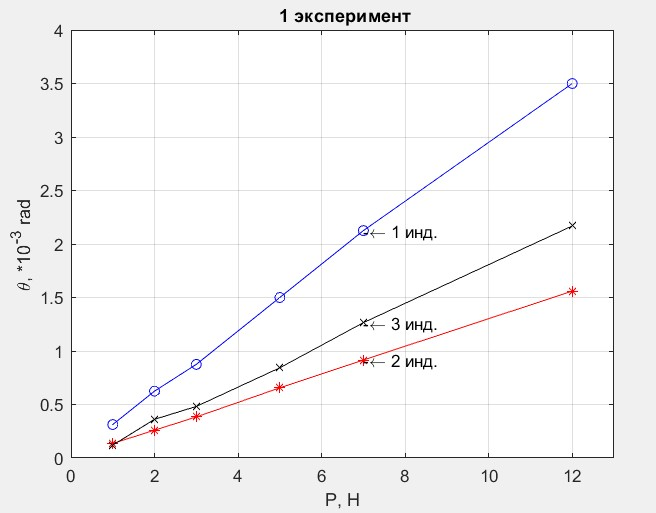
\includegraphics[width = 15cm]{teta_1.jpg}
\caption{Графики зависимости угла поворота $\theta$ от нагрузки}
\label{theta_levoe}
\end{figure}

\begin{figure}[h]
\centering
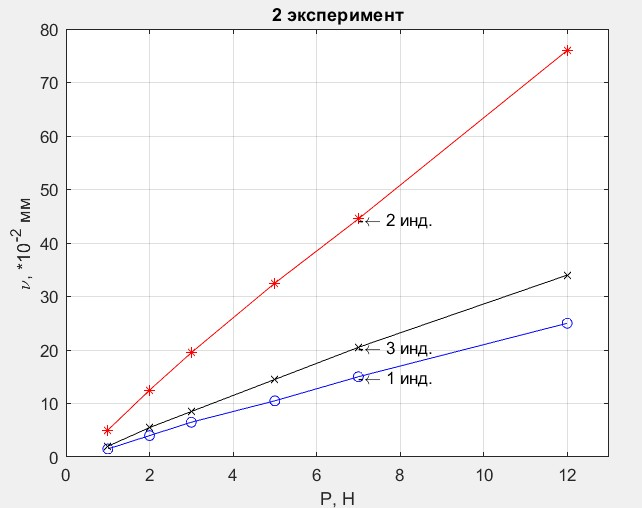
\includegraphics[width = 15cm]{nu_2.jpg}
\caption{Графики зависимости угла поворота $\theta$ от нагрузки}
\label{theta_pravoe}
\end{figure}


\end{document}
